\documentclass[11pt,a4paper]{article}
\usepackage[utf8]{inputenc}
\usepackage[T1]{fontenc}
\usepackage{mathptmx}
\usepackage{amsfonts}
\usepackage{amsmath, amssymb}
\usepackage{bm}
\usepackage{nccmath}
\usepackage{graphicx}
\usepackage{titling}
\usepackage{indentfirst}
\usepackage{url}
\usepackage{xurl}
\usepackage[backend=biber,style=apa,date=year]{biblatex}
\usepackage{csquotes}
\usepackage{float}
\usepackage{sectsty}
\usepackage{enumitem}
\usepackage{hyphenat}
\usepackage{wrapfig}
\usepackage{hyperref}
\usepackage{enumitem}
\usepackage{titlesec}
\usepackage[skip=0pt]{caption}
\setlength{\parskip}{1em}
\usepackage{tikz}
\usepackage{breakcites}
\usetikzlibrary{positioning}
\usepackage{geometry}
 \geometry{
 a4paper,
 left=25.4mm,
 right=25.4mm,
 top=25.4mm,
 bottom=25.4mm
 }
\usepackage{subcaption}

\hypersetup{
    colorlinks=TRUE, %set true if you want colored links
    linktoc=all,     %set to all if you want both sections and subsections linked
    citecolor=blue,
    linkcolor=blue,
    urlcolor=blue%choose some color if you want links to stand out
}
\DeclareSourcemap{
  \maps[datatype=bibtex]{
      \map{
        \step[fieldset=urldate, null]
      }
   }
}
\usepackage[top=0.5in, bottom=0.5in,left=1in,right=1in]{geometry} 
\subsectionfont{\fontsize{12}{15}\selectfont}
\DeclareMathSymbol{\mh}{\mathord}{operators}{`\-}
\addbibresource{Bio.bib}

%%%%%%%%%%%%%%%%%%%%%%%%%%%%%%%%%%%%%%%%%%%%%%%%%%%%%%%%%%%%%%%%%%%%%%%%%%%%%%%%%%%%%%%%%%%%%%%%%%%%%%%%%%%%



\title{Balancing Groundwater Sustainability and Agricultural Economic Goals through Evolutionary Direct Policy Search}

\author{José M. Rodríguez-Flores, Rohini Gupta, Harrison B. Zeff,  \\ Jorge Valero-Fandiño, Patrick M. Reed, Josué Medellín-Azuara}

\date{}

\begin{document}

\maketitle


\section*{Abstract}

The framework used in this study enables us to find policy strategies that are more likely accepted by stakeholders due to the heterogeneity of solutions in the Pareto-set and their robustness to uncertain surface water supplies. 
 
\section{Introduction}

As irrigation water demand increases and droughts become more frequent, agricultural regions in the world are relying more on groundwater. In Mediterranean climate regions, as California, and arid and semi-arid regions with variable precipitation, groundwater is a reliable source of water key for water security and food security (\cite{priyan_issues_2021,malmgren_groundwater_2022}). Aquifer systems flux dynamics are sensitive to changes in temperatures, precipitation and surface water flows, that are impacted with climate change (\cite{clifton_water_2010,cuthbert_global_2019}). However the largest impact from climate change is indirectly through changes in land use and water demand by human activities (\cite{taylor_ground_2013}). Globally water from aquifers account for 43 of the total consumptive water use in agriculture (\cite{siebert_groundwater_2010}), which is expected to increase as surface water scarcity increases (\cite{wada_nonsustainable_2012}). Additionally the lack of groundwater management in agriculture have lead to stress and depletion of aquifers (\cite{dalin_groundwater_2017, wada_global_2010}), affecting dependant ecosystems (\cite{bierkens_non-renewable_2019}), limiting its access to shallow water-table reliant communities (\cite{perrone_dry_2017,pauloo_domestic_2020}), reducing groundwater quality, among others. For this reason groundwater management and long-term planing is necessary to stop the groundwater depletion trajectory that has been observed globally (\cite{gorelick_global_2015}).

Multiple challenges inherent to coupled food-water systems (\cite{polhill_modelling_2016}) are present in long-term dynamic water management. First, food-water systems are dynamic, each component evolve as well as their feed-backs (\cite{filatova_regime_2016}), thus management decisions should adapt as the system evolves. Second, water management policies may result in trade-offs between economic and water sustainability objectives (\cite{mcdermid_minimizing_2021,torhan_tradeoffs_2022,young_hydrologic-economic_2021,stone_economic_2022}). Lastly, there are intrinsic uncertainties in food-water systems sometimes considered deep uncertainties or with no knowledge of their distribution (\cite{stirling_keep_2010}) that need to be accounted, including uncertain surface water supplies.  

There is a growing literature on assessing management policies and mechanisms for groundwater sustainability in agriculture. Water use and land use controls as well as economic instruments are the most common strategies that have been studied (\cite{clifton_water_2010}), such as groundwater pumping taxing and pricing (\cite{madani_exogenous_2013,mulligan_assessing_2014,stone_economic_2022}), pumping restrictions (\cite{young_hydrologic-economic_2021,lan_performance_2021,macewan_hydroeconomic_2017,rodriguez-flores_global_2022}), pricing energy (\cite{hrozencik_impacts_2022}), groundwater markets or trading mechanisms (\cite{khan_effect_2019,kuwayama_regulation_2013}), land fallowing (\cite{van_schmidt_linkages_2022}), land management (\cite{bourque_balancing_2019,li_evaluation_2018,bryant_shaping_2020}) and the combination of different strategies (\cite{graveline_combining_2019,hrozencik_heterogeneous_2017}). However most of the studies do not capture the characteristics of the coupled food-water systems and the complexity in decisions that can be made. 

Recent modeling frameworks show the benefits of dynamic adaptive policies in complex systems \cite{herman_climate_2020} show a that and the adaptive characteristics of policy decisions
Studies usually rely on assessing predefined policy instruments that can have is not able to represent the adaptive capacity of stakeholders who can adapt their decisions as changes are present in the system. Second, studies generally focus on the implementation of one policy instrument at a time which does not show the flexibility that a combination of strategies can have, particularly in irrigated agriculture where the approach may change in different water conditions. Finally, the search and assessment of the best policy instruments are usually explored under scenarios that not explore the full space of uncertainties in the system. The EMODPS framework implemented in this study addresses this limitations with a more flexible approach for the search of optimal policy instruments, assuming that water managers and farmers have a portfolio of policy strategies that can be implemented every year: groundwater pumping restrictions, groundwater pumping fee, total land use controls and perennial crops restrictions, and considering uncertainty in the search. 

In food-water systems researchers have developed a wide range of methods that serve as supporting tools for policy decision making assessment in climate change adaptation using Hydro-Economic Models (HEMs) (\cite{ward_hydroeconomic_2021}). HEMs are able to abstract farmers behaviour and hydrology dynamics, their evolution and feedback, by integrating farmers decision models with reservoirs operation models, hydrology models or hydrological response functions (\cite{harou_hydro-economic_2009}). Given the modular characteristic of these integrated methods is possible to assess multiple performance metrics that stakeholders are interested in analyze for example economic revenues from agricultural production and groundwater depth as shown by \textcite{macewan_hydroeconomic_2017}, \textcite{afshar_multi-objective_2020} and \textcite{graveline_combining_2019}. Additionally different decision making frameworks have been used in the HEMs literature to asses the performance adaptation policies under different scenarios and time-scales (\cite{waldman_agricultural_2020,robert_processes_2016}). However to investigate climate change adaptation decisions in irrigated agriculture classic programming frameworks have some limitations, including a large decision variable space for dynamic applications (\cite{taylor_applications_2019}) and complexity to incorporate both conflicting objectives and uncertainties (\cite{herman_climate_2020}). In this regard heuristic methods, as Multi-objective evolutionary algorithms (MOEAs) (\cite{coello_evolutionary_2007}) can be a better fit to represent the complexity of land and water decision making in food-water systems, which have been widely applied in reservoirs operation and environmental research (\cite{maier_evolutionary_2014}).

This study shows a novel application of HEMs and heuristic methods using a Bi-level optimization process where a agricultural production model with a groundwater depth response function is nested in a MOEA using Evolutionary Multi-Objective Direct Policy Search (EMODPS) (\cite{giuliani_curses_2016}). This process follows a parameterization–simulation–optimization process (\cite{rosenstein_robot_2001,koutsoyiannis_evaluation_2003}) where we identify adaptive policy control strategies mapped through a non linear function and which parameters are optimized along with the problem trade-offs. EMODPS makes the adaptive policy search more efficient as the structural parameters of a non-linear function are optimized instead of the policy decisions while including uncertainties in the system. The EMODPS mapping function uses information of the system state from farms and aquifer conditions to inform policy decisions showing a feed-back or closed loop control resulting in state-aware policies (\cite{giuliani_curses_2016}). Advantages of Direct Policy Search compared to classic stochastic dynamic programming methods have been shown in environmental and water allocation research (\cite{quinn_direct_2017,gupta_can_2020,macian-sorribes_inferring_2020,zatarain_salazar_balancing_2017}). Additionally the policies found in the Pareto-set can be assessed following robust planning frameworks (\cite{lempert_making_2013,herman_climate_2020,kasprzyk_many_2013}) including validating or assessing optimal policies using robustness metrics that represent stakeholders preferences (\cite{mcphail_robustness_2018,herman_how_2015}) 

and using sensitivity analysis to identify how information in the system (system-state variables) influence the selection of policy decisions over time. Finally, visualization of the results, can be used to show stakeholders about trade-offs between revenues of agriculture and to identify areas of inputs-policy decisions for further exploration. 

The present study is applied to an irrigation districts in the San Joaquin Valley, California where over-drafted groundwater basins are mandated by the state government to achieve sustainability by 2040. Groundwater sustainability agencies have developed policy strategies where decision making supporting tools as this study can be helpful in that process as the region gets in to another multi-year drought. In the next section we explain more details about the study area and problem definition. In Section 3 we describe the calibration process of the HEM, followed by the dynamic policies formulation in Section 4. In Section 5 we explain details about the algorithm and computational experiment. Results are presented in section 6, and limitations and future work. Finally we conclude with conclusions and policy implications of this work for this and other regions with groundwater overdraft in Section 7.

\section{Study area and problem definition}

The San Joaquin Valley (SJV) in California is the most important agricultural region in the United States by economic value (\cite{usda_national_2020}). The Mediterranean weather in the region and its dependence on atmospheric rivers that supplies precipitation and snow-pack make it vulnerable to drought events (\cite{espinoza_global_2018}). Additionally, increments on temperature, evapotranspiration, and reduced surface water supply are expected to exacerbate with climate change (\cite{fernandez-bou_regional_2021}).

 In recent decades the agricultural sector has been largely impacted by multi-year droughts (\cite{lund_lessons_2018,medellin-azuara_economic_2022}).  During dry periods agricultural groundwater pumping is used as a buffer to reduce the negative impacts of surface water shortages but that has led to overdraft (\cite{liu_groundwater_2022}). Over-drafted groundwater basins in the SJV show negative effects related to groundwater depletion, including land subsidence (\cite{ojha_sustained_2018}), lowering groundwater levels, reduction of groundwater storage (\cite{alam_post-drought_2021}), and degraded water quality (\cite{levy_critical_2021}).  
 
 Additionally, in the SJV there has been an expansion of perennial tree crops, mainly Almonds which is the most important commodity by value  in the region (\cite{usda_national_2020}). Although high profitable, the expansion of perennial tree crops represents a less flexible water demand and a higher financial risk to water shortages due to high establishment costs (\cite{qin_flexibility_2019,mall_water_2019}). Other important commodities in the region include vine, alfalfa, corn, cotton and cucumbers (Figure Sx). 

\subsection{Decision Making for Groundwater Sustainability}

 The Sustainable Groundwater Management Act (SGMA) (\cite{dwr_sustainable_2021}) released in 2014 requires that critically over-drafted basins achieve sustainable levels by the year 2040. Groundwater Sustainability Agencies (GSAs) are responsible to develop and enforce policies to manage the conjunctive use of water that address groundwater sustainability goals, including a sustainable groundwater depth level. The state defined the guidelines and practices in the Sustainable Management Criteria (\cite{dwr_sustainable_2017}), that GSAs can use to develop strategies defined in their sustainability plans (available in the \hyperlink{https://water.ca.gov/Programs/Groundwater-Management/SGMA-Groundwater-Management/Groundwater-Sustainable-Agencies}{SGMA Portal}). This criteria defines a minimum threshold and a measurable objective (Appendix x) where for the case of achieving a sustainable groundwater level means reaching the measurable objective while allowing the groundwater level go bellow this point but not beyond the minimum threshold where undesirable results may ocurr. The buffer between the measurable objective and the minimum threshold represents a margin of operational flexibility (Figure Sx), where GSAs can manage groundwater in a flexible way between dry and wet years.  
  
This study area of this study is the Semitropic Water Storage District (SWSD), located in the SJV and Kern County groundwater basin (Figure 1). The SWSD also operates its own Groundwater Sustainability Agency. As mentioned in the introduction the objectives of this study are twofold. First, to asses EMODPS as a modeling tool to identify adaptive strategies to achieve groundwater sustainability accounting for the characteristics of the food-water system. Second, to asses the performance of the policies within the context of the Sustainable Groundwater Management Criteria and the trade-offs between groundwater sustainability and economic revenues from food production. The four possible strategies analyzed in this study are: a groundwater use controls and a groundwater pumping fee, that can be implemented by the GSA, and a total land use and the perennial crops planting decisions, operated by farmers. Other policies as water market mechanisms and supply-side policies focused on incrementing groundwater storage, such as Managed Aquifer Recharge (MAR) (\cite{ulibarri_assessing_2021}) are out of the scope of this study. 

\begin{figure}[H]
    \centering
    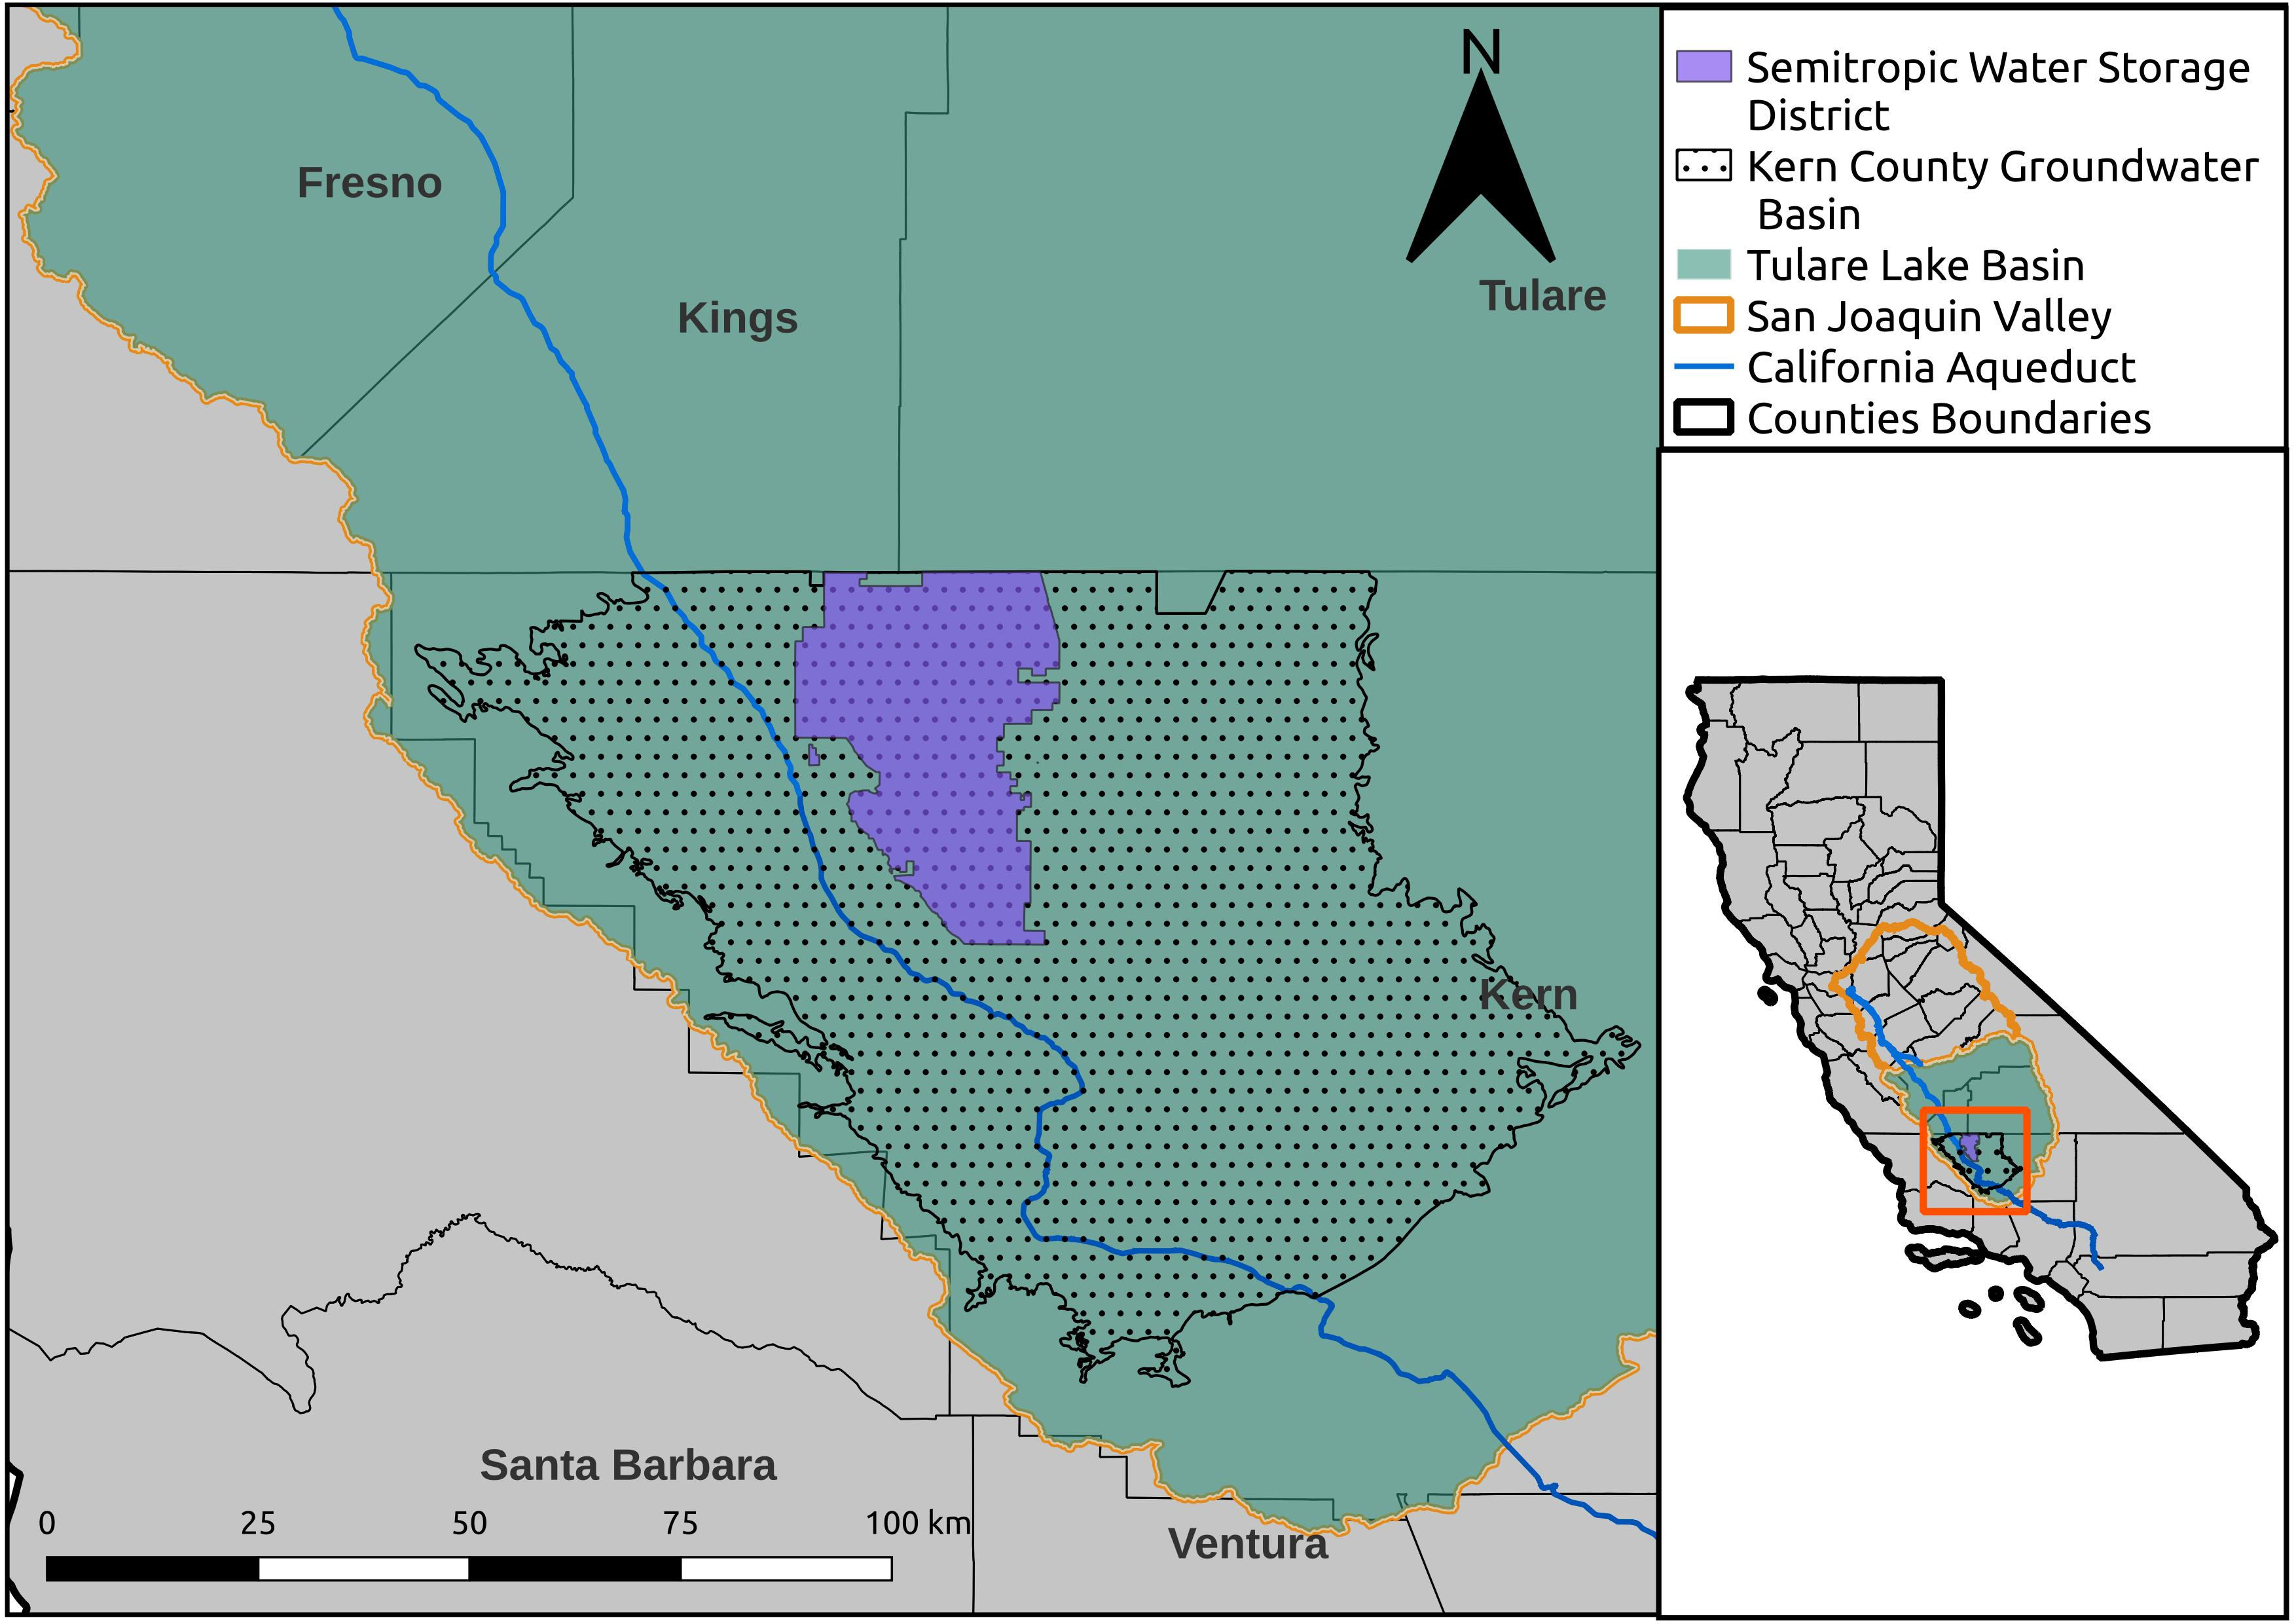
\includegraphics[width=0.8\textwidth]{Map_Semitropic.jpg}
    \caption{Semitropic Water Storage District located in the San Joaquin Valley, California}
    \label{fig:1}
\end{figure}

\section{Hydro-Economic model}

As explained in Section 1.1 given the Sustainable Groundwater Management Act GSAs and Water Agencies need to implement policies that achieve this while achieving the economic goals of agriculture. We analyze the trade-offs between keeping the groundwater potentiometric level, as a proxy to groundwater sustainability, and agricultural economic revenues. The Hydro-economic model has multiple inputs every time step, including land and water allocation by crop, however to analyze the implementation of groundwater management revenues we focused on two main outputs: revenues and groundwater depth. Implementing groundwater sustainability strategies and based on the objectives defined in the next sections. All the objective values are estimated from the policy decision created by the dynamic policy search that inputs to the Hydro-economic model, from which we use the outputs as defined in the Section 3.

\subsection{Economic model}

The food production system was modeled using a hydro-economic model (\cite{harou_hydro-economic_2009}) able to represent a yearly net profit maximization for each irrigation district where farmers make land and water (surface and groundwater) allocation decisions to each crop. This maximization problem assumes that farmers take with changing conditions including crop prices, surface water availability, price of surface water, price of electricity and policy decisions. We used a mathematical model based on Positive Mathematical Programming (PMP) (\cite{howitt_calibration_1995}), using a stochastic data assimilation method to calibrate the economic parameters described by \textcite{maneta_stochastic_2014} and \textcite{maneta_satellite-driven_2020}. This calibration framework enables updating the distribution of the calibration parameters every time data becomes available. 

With the PMP calibration using a stochastic data assimilation we address two objectives: avoid the assumption that farmers will behave as a particular year (if calibrating to only one year or average of years) but rather capturing the mid-term behaviour, and second we account for the uncertainty in the calibration parameters inherited from uncertain inputs and observations in used the calibration. Additionally this stochastic framework enables to update the distribution of parameters as new observations become available. We adapted the Python code used in \textcite{maneta_satellite-driven_2020} that uses a Monte Carlo recursive Bayesian estimator based on the ensemble Kalman Filter (enKF) (\cite{evensen_sequential_1994}). The enKF uses uses the calibration conditions (Appendix A) to recursively update the distribution of the parameters using historical data on crop production, land use, water use, own-price supply elasticities, crop yield response to water and production costs. The optimally conditions to perform the stochastic assimilation are following the PMP calibration described by \cite{merel_fully_2011}, which uses using a generalize Constant Elasticity of Substitution (CES) production function as a convex production function and the calibration of the Lagrange multipliers use in the linear costs of land and water explained by \textcite{garnache_calibration_2017}. Details about the calibration process, data sources and specific parameters used in the calibration refer to Appendix A. 

\sloppy After the last year of historical observation was used in the data assimilation process we used the resultant ensemble of size 400 for the calibration parameters $\theta_{i} = [\mu_{i},\beta_{i,water},\beta_{i,land},\delta_{i},\lambda_{i,land},\lambda_{i,water},\bar{\lambda}_{land}]$ in the economic model (Equations 1-7 ). Using a sample of the distribution of the calibration parameters and a year t state of the world (Section 3.3) of surface water supply, crop prices, electricity price and surface water price, the economic model solves the following maximization problem, irrigation district index and sample index for the parameters in $\theta$ were excluded for simplicity:

\begin{alignat}{1}
\underset{{\substack{x_{i,land,t}\geq0\\x_{i,water,t}\geq0\\wat_{i,w,t}\geq0}}}{max}& \sum_{i} \{p_{i,t} \mu_{i}(\beta_{i,land} x^{\rho_i}_{i,land,t}+\beta_{i,water} x^{\rho_i}_{i,water,t})^{\delta_{i}/\rho_i} - (\omega_{i,land} + \lambda_{i,land} + \bar{\lambda}_{land}) x_{i,land,t} \notag \\&-(\omega_{SW,t}+ \lambda_{i,water} )wat_{i,SW,t} - (\omega_{GW,t}+ \lambda_{i,water} + u^{GWF}_{t})wat_{i,GW,t}\}
\end{alignat}

\textit{subject to}
\begin{flalign}
&\sum_{i} x_{i,land,t} \leq u^{TL}_{t}& \\
&\underset{i\in{PC}}{\sum} x_{i,land,t}  \leq  u^{PL}_{t}\\
&\underset{i\in{PC}}{\sum} x_{i,land,t}  \geq \underset{i\in{PC}}{\sum} x_{i,land_{t\mh1}} * 0.95 \\
&x_{i,water,t} = wat_{i,SW,t} + wat_{i,GW_t} \\
&\sum_{i} wat_{i,SW,t} \leq b_{SW,t}   \\
&\sum_{i} wat_{i,GW,t} \leq u^{GWP}_t \\
& x_{i,water,t} \geq \bar{x}_{i,water}*0.95
\end{flalign}

Equation 1 represents the net revenue that is maximized by allocating land $x_{land,i}$, total water $x_{water,i}$, surface water $wat_{SW,i}$ and groundwater $wat_{GW,i}$ to each crop i (Figure A.1). $p_{i,t}$ is the price of crop $i$. Crop production in the first term of Equation 1 is represented by a CES production function, where $\beta_{i,j=[land,water]}$ are the relative use of inputs, a scale parameter $\mu_{i}$, $\rho = (\sigma-1)/(\sigma)$ where $\sigma = 0.17$ is the elasticity of substitution parameter and $\delta$s are calibrated using the first order conditions. The rest of the parameters used in the linear costs are the calibrated Lagrange multipliers $\lambda_{water},\lambda_{land}$, associated to the observed water allocation per crop and land allocated per crop constraints respectively (Appendix A). Variable costs are represented by a linear cost as a function of land and water allocated, where $\omega_{i,land}$ is the cost of land, price of surface water per unit of water $\omega_{SW,t}$, the volumetric unit cost groundwater pumping $\omega_{GW,t}$ is a function of price of electricity ($\omega_{E,t}$), the groundwater depth or potentiometric level ($GWD_t$) and other parameters related to the characteristics of the wells (Appendix A.2). Additionally a per cubic meter $u^{GWF}_{t}$ pumping fee can be implemented that sums to the pumping cost. The maximization problem is subject to resources availability and land and water quantitative controls. Equation 2 is a total land restriction where $u^{TL}_{t}$ is the policy that can be implemented in a year $t$. Equation 3 is an upper boundary perennial crops policy restriction $u^{PL}_{t}$ that levers the expansion or reduction of land allocated to perennial crops, where $PC \in$ \{Almonds and Pistachios, Subtropical, Other Deciduous and Vine\}. Surface water availability $b_{SW,t}$ (Equation 6). Equation 7 is the total groundwater pumping restriction where $u^{GWP}_{t}$ is the maximum allowed groundwater pumping policy.  All decision policies implemented every year $t$ are explained more in detail in section 3.1.

\subsection{Groundwater Depth Response Function}

Groundwater in the San Joaquin Valley is a complex system, its dynamics depend on many geological, hydrological, climate and human components. Including the seepage from stream inflows, lateral flows, aquiclude, pumping for urban and agricultural use, and managed aquifer recharge. To incorporate the dynamics of groundwater level (potentiometric level) we used outputs from the physical based model Fine Grid California Central Valley Groundwater-Surface Water Simulation Model (C2VSIM-FG) (\cite{brush_users_2013}). C2VSIM-FG has a finite element grid of more than 35,000 elements for all the Central Valley California (Sacramento Valley and San Joaquin Valley), for each element is able to link land surface, surface water and groundwater. The model uses historical data on cropland use, crop water demand, surface water diversions, precipitation, soil moisture, among others. C2VSIM-FG can be run for a simulation period from 1973 through 2015 at a monthly time step. After the simulation creates water budget, that include agricultural supply requirement, surface water deliveries, groundwater pumping, change in groundwater storage, groundwater depth, among others by element. Water budget outputs can be post-processed to create water budgets for defined boundaries (group of elements) of for example irrigation districts. C2VSIM-FG has been used by GSAs and Irrigation Districts to develop their sustainability plans.

For this study we ran C2VSIM-FG and created water budgets for the boundaries of Westlands WD and Semitropic WSD. We used the weighted-average potentiometric level, of all the aquifer layers, to agricultural groundwater pumping for all the nodes within the district boundaries. Weighting the aquifers depth to agricultural pumping allow us to remove the nodes where there is not agriculture. Since the economic model simulates farmers decisions at a yearly time step we used the groundwater depth level at the beginning of water year (October) end of the water year (September), and the total groundwater pumping in the water year. Figure 2 shows the simulated groundwater depth and agricultural pumping from C2VSIM-FG at the end of the water year. 

\begin{figure}[H]
    \centering
    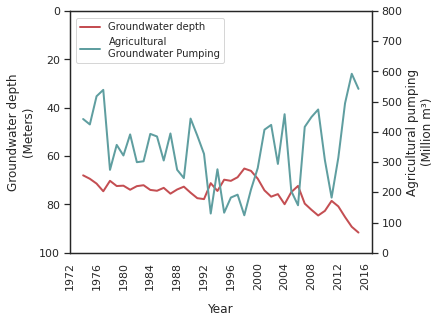
\includegraphics[width=0.5\textwidth]{c2vsim_semitropic.png}
    \caption{Groundwater depth and agricultural groundwater pumping from simulation outputs of C2VSIM-FG}
    \label{fig:mes1h1}
\end{figure}

To incorporate the feedback between groundwater depth and agricultural pumping we use the difference (groundwater depth change) between the groundwater depth level at the beginning of the irrigation season and average groundwater depth level at the end of the irrigation season. We used different variables to select the best model configuration that predicts groundwater depth change at the end of the year t ($\Delta GWD_{t}$): Groundwater Pumping in the year t ($GWP_{t}$), Groundwater Pumping in the year t-1 ($GWP_{t-1}$) to include the possible auto-correlation, an intercept, and water year Type of year t ($WY_{t}$) and water year type of year t-1 ($WY_{t-1}$) as index variables. We used three water year type categories: Wet, Normal and Dry. Normal category includes above and bellow normal categories and Dry water year includes Critical and Dry types, all of them are defined by the Water Year Hydrologic Classification Indices of the California Department of Water Resources (\cite{dwr_california_2020}). As shown by \textcite{macewan_hydroeconomic_2017} using the water type variable we can capture information related to hydro-logical processes that shift how agricultural pumping affect groundwater depth levels. Depending on the water conditions in a year changes in surface water is available, hence the demand of groundwater, and other hydrological processes as run off and seepage to the groundwater change. 

We use Bayesian inference to fit different model variations. Bayesian inference provides advantages over other statistical frameworks, since it quantifies the uncertainty of the prediction accounting for uncertainty in the the parameters (\cite{mcelreath_statistical_2020}). Additionally when new information becomes available the parameters distributions can be updated. Different model variations were fitted to compare how information informs the best to the groundwater depth change prediction, including pooled, un-pooled and hierarchical models. Refer to Appendix B for detailed information about the model selection process. Models were fit using a Markov Chain Monte Carlo (MCMC) sampling method using the probabilistic programming Python package PyMC (\cite{salvatier_probabilistic_2016}). Model selection was done using the Leave-one-out Cross-validation (LOO-CV) as estimate of the out-of-sample predictive fit (\cite{vehtari_practical_2017}), selecting the model with the highest log-scale LOO-CV or with he best out-of-sample prediction was selected for each district.

Using the model with the best best out-of-sample predictive fit for each district Figure 3 shows the median of the simulated posterior predictive groundwater depth change for Semitropic (left) and Westlands (right). We can observe that in general the response function for both districts the response function can predict correctly the groundwater depth change, with an $r^2 = 0.90 (r^2 std = 0.007)$ for SWD. Even-though the fit of the response function to the simulation results from C2VSIM-FG is reasonable this model does not fully represents the complexity of the groundwater system, since does not account for all the dynamics of groundwater in the aquifer such as lateral flows.

\begin{figure}[H]
    \centering
    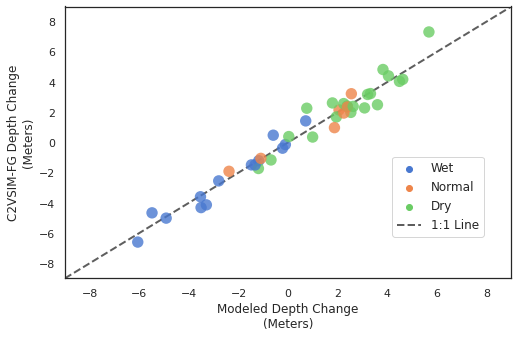
\includegraphics[width=0.5\textwidth]{results_gw_depth_response_calib.png}
    \caption{Results groundwater depth response function. Dots are the median of each posterior predictive distribution of groundwater depth change, colors represent water-year type categories in year t.}
    \label{fig:mesh1}
\end{figure}

Every year step the groundwater depth change response functions are used to predict every year t the groundwater depth at the end of the irrigation season. Equation 8 shows how the ground water depth level ($GWD_{t}$) at the beginning of the year t calculated as the sum of the groundwater depth level at the beginning of the year t-1 ($GW_{t-1}$) and the median of the predictive posterior distribution for groundwater depth change ($\overline{\Delta GWD}_{t-1}$) at the end of the year t-1. By embedding the hydrologic response in to the economic model and by using the cost of pumping as a function of the groundwater depth we are able to model the feed-back between agriculture production and groundwater system at a yearly step.

\begin{align}
GWD_{t} = GWD_{t-1} + \overline{\Delta GWD}_{t-1}
\end{align}

\subsection{Stochastic time series}

In order to run the model dynamically we build Monte Carlo time series for economic and hydrologic conditions that feed the Hydro-economic model. Each time series starts at $t_{0}=2016$. In our analysis we included the Climate Change effects to surface water supplies using surface water deliveries $b_{SW,t}$ to the irrigation district using the California’s Food-Energy-Water System simulation model (CALFEWS) (\cite{zeff_californias_2021}), these were simulated with down-scaled data from the Coupled Model Intercomparison Project 5 (CMIP5). Seven of the ten Global Circulation Models (GCMs) suggested by \textcite{pierce_climate_2018} were used in this study: CCSM4, MIROC5, CanESM2, CNRM-CM5, GFDL-CM3, HadGEM2-CC and HadGEM2-ES (Figure 4) using the Representative Concentration Pathway (RCP) 4.5 and 8.5. This study does not account on changes to crop yields from climate change which can be affected by changes in temperature and levels of $CO_{2}$ due to the lack of information. 

Additionally each time t we considered uncertainties on economical variables and calibration parameters of the PMP model.  Crop prices $p_{i,t}$ were sampled using the historical data from 1980 to 2020 (\cite{usda_national_2020}), price of electricity ($\omega_{E,t}$) was sampled from the historical (2008-2021) reported by the Pacific Gas and Electricity Company (PG\&E) for small and large agricultural users. Price of surface water ($\omega_{SW,t}$) was sampled from rates reported in different water-year types using surface water supply to define the water-year type category. From the last parameters distribution in the last data assimilation step (Appendix A). Each time step a sample from the posterior distribution of the calibration parameters $\theta_{i}$ was sampled. Sources of data used to build the Monte Carlo time series are summarized in Table 1. 

\begin{center}
\begin{tabular}{ |c|c|c|c| } 
 \hline
 Variable & Symbol & Units & Source \\ 
 \hline
 Crop prices & $p_{i}$ & \$/ton & \textcite{usda_national_2020}\\
 Price of electricity & $\omega_{E,t}$ & $\$/Kwh$ & \textcite{pge_pacific_2021} \\
 Price of surface water & $\omega_{SW,t}$ & $\$/m^3$ & Irrigation districts reports\\
 Surface water supply & $b_{SW,t}$ & $m^3$ & \textcite{zeff_californias_2021}\\
 Calibration parameters & $\theta_i$ & - & Calibration process \\
 \hline
 \end{tabular}
\captionof{table}{Data Sources for Monte Carlo Time Series}
\end{center}

\begin{figure}[H]
    \centering
    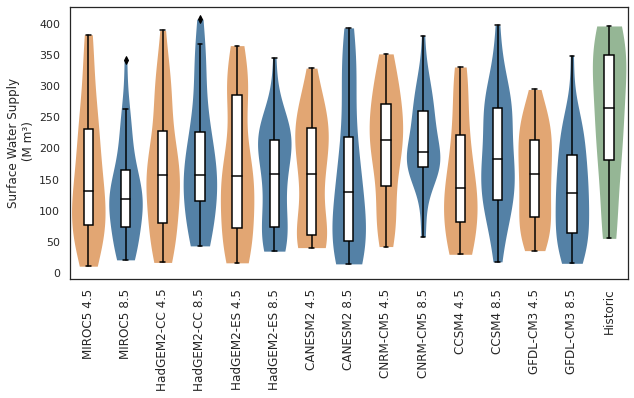
\includegraphics[width=0.7\textwidth]{gcm_surface_water.png}
    \caption{Distribution of historical (1999-2015) and surface water deliveries from CALFEWS (2016-2045) used in this study} \label{fig:SWSemitropic}
\end{figure}

\section{Dynamic Adaptive Policy Strategies}

These trade-offs repres stakeholders. Solutions may result in a set of solutions, rather than in a unique or optimal solution characterized in a Pareto-set or trade-off curve (\cite{greening_design_2004,null_pareto_2021}), where decision makers can visualize and understand trade-offs of possible policies.

Farmers and water managers include new information of the system in to their decision making process.

The policy search consist on assessing candidate policies through a direct policy search simulated in the Hydro-economic model (Equations 1-10). Different land use and water use controls and economic instruments can be implemented by water managers: Groundwater pumping fee (GWF), total land restriction (TL), perennial cropland restriction (PL) and groundwater pumping restriction (GWP). Decisions are simulated by a control policy that defines the combination and magnitude of the four decisions to be taken every year. Given the variability of surface water supply, farmers crop-land decisions, and aquifer's depth at the beginning of the irrigation season, decisions can be adapted. For this reason we use direct policy search, a closed-loop method, where each time step dynamic policies are informed by system-state information variables. 

With EMODPS we optimize the structural parameters of a parametric function instead of optimizing the policy decisions reducing the number of decision variables that other problem formulations as stochastic dynamic programming can have. Control policies can be represented by different  parametric functions, including linear, polynomial, artificial neural networks, decision trees and radial basis functions \cite{giuliani_universal_2014}, which structures are used to map system-state variables policy decisions. In this study we use Cubic Radial Basis Functions (RBFs) to represent the complexity of dynamic cropland and groundwater policies decision making. Searching for optimal RBFs structural parameters using MOEA allows us to dynamically map system state variables of the food-water system to policy decisions while achieving multiple objectives.

\subsection{Direct Policy Search}

Dynamic land and groundwater management decisions made at every year step $t$ are represented by the vector $u_{t}^D$ where $D \in \{GWP,TL,PL,GWF\}$ represent each of the four possible decisions. The set of decisions in Equation 11 equals to the outputs of a policy $P^D$ which is a mathematical function with two vector inputs: the structural parameters of the RBFs $\psi^D$ and system-state information vector $I_{t'}$. Information variables in $I_{t'}$ represent key components of the food-water system which values can be from the current year $t$ or previous year $t-1$. 

\begin{align}
u_{t}^D = P^{D}(I_{t'}|\psi^{D})
\end{align}

In direct policy search, a closed-loop policy method, RBFs have shown to be an efficient way to represent complex policy decisions (\cite{busoniu_cross-entropy_2011}). These have been applied in several applications to environmental, water allocation and reservoir operation problems (\cite{giuliani_universal_2014,gupta_can_2020,quinn_direct_2017,garner_using_2018, zatarain_salazar_balancing_2017}) showing as well flexibility to incorporate uncertainty and multiple objectives. For this study we define the mapping policy decision function $P^D$ as set of cubic radial basis functions as shown in Equation 10.

\begin{align}
u_{t}^D = \phi^{D}\left(\sum_{m=1}^M w_{m}^D \sum_{j=1}^J \left\lvert\dfrac{[I_{t'}]_{j}-c_{j,m}}{r_{j,m}}\right\rvert^{3}\right)
\end{align}

Where $\phi^{D}$ is an outer function, $w_{m}^D$ is the weight of M cubic radial basis functions. The weights are chosen within the boundaries $ 0 \leq w_{m} \leq 1$ and subject to $\sum_{m=1}^M m_{m}^D= 1$. The four decisions share the RBFs structure in the control policy; hence the information vector $I_{t'}$ is shared for all decisions. This vector represents system state variables that inform the policies, where $\overline{GWD}_{t}$ is the normalized level to groundwater at the beginning of the year, $\overline{PCT}_{t-1}$ is the normalized area devoted for perennial crops production in the year $t-1$ and $PCT_{t-1}=\sum_{i \in PC}x_{i,land,t-1}$ . $\overline{b}_{SW,t}$ is the normalized surface water available in year $t$. Normalization was performed using $k^{GWD}$, $k^{TL}$, $k^{SW}$ to obtain $\overline{GWD}_{t}$, $\overline{PCT}_{t-1}$, $\overline{b}_{SW,t}$ respectively summarized in Table 2. $c_{j,m} \in [-1,1]$ and $r_{j,m} \in (0,1]$ are the center and radius respectively shared by all the RBFs.

\begin{align}
I_{t'} = [\overline{GWD}_{t},\overline{PCT}_{t-1},\overline{b}_{SW,t}]
\end{align}

The function $\phi^{D}$ in Equation 10 can consist on two functions, unnormalize $\phi^{D,N}$ and constraint $\phi^{D,C}$, applied to obtain the values of groundwater management decisions in the control policy $u_{t}^D$. Being $z_{t}$ the argument in the $\phi^{D}$ function the value of each decision is defined by the following equation.

\begin{align}
u^{D}_t = \phi^{D,C}(\phi^{D,N}(z_{t}))
\end{align}

For the groundwater pumping restriction policy ($u^{GWP}_t$) $\phi^{GWP,N}$ scales the groundwater that farmer will have available between zero and the pumping capacity of the district $k^{GWP}$. $\phi^{GWP,C}$ constraints the groundwater pumping to be at least the difference between the water demand by perennial crops of the year $t-1$ and the surface water available in the year $t$. 

\begin{align}
z'_{t}=\phi^{GWP,N}(z_{t}) = k^{GWP}max(min(z_{t},1),0) 
\end{align}

\begin{align}
u^{GWP}_t = \phi^{GWP,C}(z'_{t})= max(z'_{t},\underset{i \in PC}{\sum} x_{i,water_{t\mh1}} - \; b_{SW,t})
\end{align}

Next, $\phi^{TL,N}$ scales the total land available that farmers can produce in the district for the year t, between zero and $k^{TL}$, where $k^{LR}$ is the total land in the district. $\phi^{TL,C}$ constraints the total land available to be at least the land used by perennial crops in the the year $t-1$.

\begin{align}
z'_{t} = \phi^{TL,N}(z_{t}) = k^{TL}max(min(z_{t},1),0)
\end{align}

\begin{align}
u^{TL}_t = \phi^{TL,C}(z'_{t})= max(z'_{t},\underset{i \in PC}{\sum} x_{i,land_{t\mh1}})
\end{align}


For the perennial crops land policy ($u^{PL}_t$), $\phi^{PL,N}$ scales the total land that can be allocated to perennial crops between zero and the total land available in the district ($k^{TL}$). $\phi^{PL,C}$ constraints the perennial restriction to be at leas 5\% of the year $t-1$ total perennial cropland, \textit{i.e} $u^{PL}$ levers the expansion or reduction of land allocated to perennial crops, if the policy reduces perennial land this cannot be less than 95\% of the previous year, and it limits the expansion of perennial crops to 5\% more acreage to the previous year $t-1$. See in Equation 4 that the upper boundary for perennial crops removal of 5\% exists in any case to ensure that solutions of the optimization model are realistic to what is the observed year to year trees removal in the region.

\begin{align}
z'_{t} = \phi^{PL,N}(z_{t}) = k^{TL}max(min(z_{t},1),0)
\end{align}

\begin{align}
u^{PL}_t = \phi^{PL,C}(z'_{t})= \begin{cases}
      \underset{i\in{PC}}{\sum} x_{i,land_{t\mh1}}*1.05,  \text{\; if \, $z'_{t}$  $>$ $\underset{i\in PC}{\sum}x_{i,land_{t\mh1}}*1.05$}\\
       \underset{i\in PC}{\sum} x_{i,land_{t\mh1}}*0.95, \text{\; elif \, $z'_{t}$  $<$ $\underset{i\in PC}{\sum}x_{i,land_{t\mh1}}*0.95$}\\
      z'_{t}, \text{\; $otherwise$}
\end{cases}     
\end{align}

Finally for the pumping fee policy ($u^{GWF}_t$), the function $\phi^{GWF}$ consits of a scaling function $\phi^{GWF,N}$ where the groundwater pumping fee can have values [0,$k^{GWF}$], $k^{GWF}$ is set to be $\$0.4/m^3$, hence the upper boundary of the pumping fee is 0.4 USD dollars per cubic meter. This fee sums to the groundwater pumping cost in the objective function of the PMP model (Equation 1).

\begin{align}
u^{GWF}_t = \phi^{GWF,N}(z_{t}) = k^{GWF}max(min(z_{t},1),0)
\end{align}

The dynamic control policy is represented by Equations 11 to 18, where the vector of structural parameters $\psi = [w^{D},c,r]$ is optimized (Section 3.2). Since the information vector $I_{t'}$ of size $J$ is shared across decisions in $M$ number of RBF's the vectors of centers (c) and radii (r) are equal to $c=[c_{0,0},...,c_{J,M}]$ and $r=[r_{0,0},...,r_{J,M}]$.


\begin{center}
\begin{tabular}{ |c|c|c|c| } 
 \hline
 Variable & Symbol & Units & Value \\ 
 \hline
 Normalization for cropland  & $k^{TL}$ & $Kha$ & 62\\
 Normalization for groundwater pumping & $k^{GW}$ & $M m^3$ & 732 \\
 Normalization groundwater depth  & $k^{GWD}$ & $m$ & 167 \\
 Normalization for pumping fee   & $k^{GWF}$ & \$/$m^3$ & 0.49 \\
 Normalization surface water  & $k^{SW}$ & $M m^3$ & 407 \\
 \hline
 \end{tabular}
\captionof{table}{Normalization factors for the decisions in the control policy}
\end{center}


\subsection{Bi-level Optimization Problem}

This study implements two optimization processes (Figure 5). In the first level a Multi Objective Evolutionary Optimization process is performed that assess candidate policies optimized over the vector of structural parameters $\Psi$ (Equations 9 - 19). Control policies $u^{D}$ are implemented in the Hydro-economic model (second-level) where the economic model is optimized and its feedback with the groundwater depth is simulated each time step $t$. Different uncertainties are considered (Section 2.3) to create a Monte Carlo ensemble of size N, where each element in the ensemble represents a time series of T years. Each time series containing surface water supplies, crop prices, electricity prices, surface water prices and calibration parameters that feed the economic model. Hence each candidate policy is evaluated across N realizations with T years. The results of this process are aggregated in five performance metrics, representing the groundwater sustainability and economic goals of each irrigation district, that feedback as objectives and constraint to the MOEA. 

\begin{figure}[H]
    \centering
    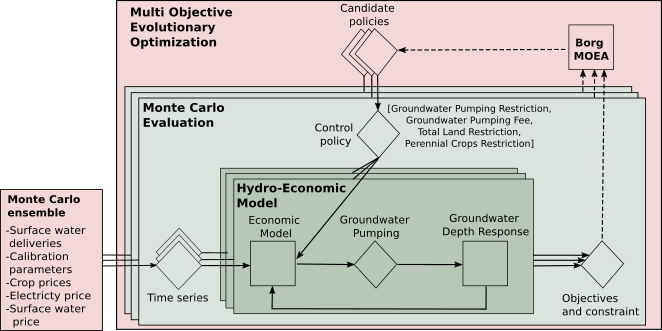
\includegraphics[width=0.9\textwidth]{Diagram2}
    \caption{Bi-level optimization problem schematic adapted from \textcite{hamilton_stream_2022}. Rectangles represent the modules that contain optimization and simulation models (squares) and inputs/outputs (diamonds). Dashed arrows depict the Borg MOEA feed-back process where the values of objectives and constraint are from performance metrics of the Hydro-economic model result of an implemented control policy.}
    \label{fig:m1esh1}
\end{figure}

As explained above the first level optimization consists in a multi-objective evolutionary optimization where five objectives are minimized or maximized, the decision variables are the structural parameters of the RBFs in the vector $\Psi$, used to parameterize the control policy. 

\begin{align}
\underset{\Psi}{argmin} = (-O_{1}(\Psi),O_{2}(\Psi),-O_{3}(\Psi),O_{4}(\Psi),-O_{5}(\Psi))
\end{align}

The first objective ($O_{1}$) is to to maximize the average total revenues $\pi_{n,t}$ from the total net revenue of N ensemble realizations with T years. This objective represents the economic objective of farmers, taken into account by water managers to make policy decisions that allow profit maximization. Since multiple policies can be applied in the EMODPS control policy, extreme policies where all controls and pumping fee are being applied can result in scenarios where revenue can be greatly affected, for this reason a lower boundary constraint for this objective to achieve an average total revenue greater or equal than \$11 billions.

\begin{align}
O_{1} = \frac{1}{N}\sum_{n=1}^N(\sum_{t=1}^T \pi_{n,t})
\end{align}


\begin{align}
O_{1} \geq 11
\end{align}

The second objective is the minimization of the average average groundwater depth. The average of groundwater depths is taken over the T years for each Monte Carlo realization, and then the average of these are taken over all the N Monte Carlo realizations. This metric represents the sustainability goal stated by SGMA, using groundwater level as a proxy of sustainability, where water managers want to minimize the distance to the groundwater (potentiometric level).

\begin{align}
O_{2} = \frac{1}{N}\sum_{n=1}^N(\frac{1}{T}\sum_{t=1}^T GWD_{n,t})
\end{align}

The third objective is to minimize the 5th percentile of minimum profits. This metric represents a \textit{max-min} goal, used to inform decision makers about the of the worst profits in a given year $t$ in Monte Carlo sample. Even though, there are many factors included in the stochastic ensemble that can be drivers of low economic revenues, water and land management policies can be a main driver, as shown by . Water managers would likely allow farmers to keep. The Q5 operator in Equation 22 takes the 5th percentile of this minimum revenue year over all the Monte Carlo ensemble. 

\begin{align}
O_{3} = Q5_{N} \bigg[\underset{t\in(1,...,T)}{min}[\pi_{n,t}]\bigg]
\end{align}

The fourth objective is to minimize the 95th percentile of maximum groundwater depths. This objective represents a \textit{min-max} goal of the highest distance to the groundwater (or worst overdraft).  The maximum groundwater depth level is taken over each ensemble of T years and the Q95 operator takes the 95th percentile over all N Monte Carlo ensemble realizations. 

\begin{align}
O_{4} = Q95_{N} \bigg[\underset{t\in(1,...,T)}{max}[\overline{\Delta GWD}_{t-1}]\bigg]
\end{align}

During dry years the distance to groundwater can increase above the sustainable level, expecting that in wet years it will recover; however water managers seek to maximize the number of years that the groundwater depth is at a sustainable level. The fifth objective is to maximize the average fraction of years (reliability) that the distance to the groundwater depth is lower or at the reference sustainable level $GWD^{SGMA}$. Additionally we included a constraint  that the reliability has to be at least 20\% (Equation 27). 

\begin{align}
O_{5} = \frac{1}{NT}\sum_{n=1}^N(\sum_{t=1}^T \tau_{n,t})\; where\; \tau_{n,t} = \begin{cases}
      1, \text{\; $GWD_{n,t}$  $\leq$ $GWD^{SGMA}$}\\
      0, \text{\; $GWD_{n,t}$ $>$ $GWD^{SGMA}$}\\
\end{cases}      
\end{align}


\begin{align}
O_{5} \geq 0.2
\end{align}


\subsection{Optimization Algorithms}

Even though direct policy search is computationally efficient the search of optimal RBFs parameters can result in a non-linear and non-convex problem (\cite{giuliani_curses_2016})  that can be solved using heuristic methods. MOEAs are stochastic search tools that perform an iterative process using evolutionary strategies inspired from nature to evolve and to improve a population of possible solutions, evaluating multiple objective functions, until a population reach a Pareto front or non-dominated solutions (\cite{coello_evolutionary_2007}). Additionally land and water management policies for the adaptation to climate change in irrigated agriculture show trade-offs across performance metrics resulting in a non-convex problem with multiple solutions where heuristic methods can be applied for their optimization (\cite{maier_evolutionary_2014, memmah_metaheuristics_2015}).  

For this study we use the Borg MOEA (\cite{hadka_borg_2013}), a self adaptive algorithm that uses probabilistic operators as $\epsilon$-dominance, adaptive population sizing and time continuation through $\epsilon$-progress. Borg MOEA has shown have better time efficiency, scalability and controllability, as well as less sensitive to its parameterizations compared to other MOEA algorithms (\cite{reed_evolutionary_2013}).  These characteristics and its support to different parallelization variants makes it widely applicable to complex problems with different scales and computational demands (\cite{hadka_large-scale_2015}), particularly in environmental (\cite{kravits_multi-objective_2021,ward_confronting_2015,meysami_evaluating_2020}), water operation (\cite{zatarain_salazar_balancing_2017,yan_many-objective_2017,smith_many-objective_2016,zeff_cooperative_2016, gupta_can_2020}), financial (\cite{hamilton_stream_2022}) and infrastructure applications (\cite{eckart_multiobjective_2018,bakhshipour_toward_2021,gold_power_2022}).   

The second level optimization, the economic model (Equations 1-7) is solved using the Python package Pyomo (\cite{hart_pyomo_2011}) and the non-linear programming solver IPOPT (\cite{wachter_implementation_2006}). The economic model decision variables are the allocation decisions of land, total water, surface water and groundwater by seventeen crop groups resulting in 68 decision variables each time step $t$ for each district. Additionally at each time step a posterior predictive sample of groundwater depth change with 400  samples is estimated using the model and trace generated in the calibration process (Section 2.2).

\section{Computational Experiment}

To find the EMODPS policy strategies we perform the bi-level optimization process for an ensemble of N = 100 Monte Carlo realizations and T = 30 years for 80,000 candidate policy trial. A structure of M=4 RBFs (Equation 10) was selected resulting in 40 decision variables in the vector $\Psi$ to be optimized in the MOEA. Since Borg MOEA is a stochastic algorithm we estimate Pareto-front solutions using five different random seeds using the master-worker parallel configuration of Borg (\cite{hadka_large-scale_2015}). $\epsilon$-values (resolution) for each objective, boundaries for weights, centers and radii and the Borg MOEA parameter values are summarized in SI Table S1. The solutions were selected from combining the solutions from different seeds and choosing the best ones. The best known Pareto set across the seeds was selected to continue the assessment its non-dominated solutions. These solutions were assessed in a larger set of Monte Carlo ensemble of N = 500 to asses their performance in more scenarios than the original sample size. These results were used to inform the robustness and sensitivity analysis.

\subsection{Robustness Analysis}

Solutions in the Pareto front are heterogeneous control policies with different levels of trade-offs among objectives from which stakeholders preferences can be incorporated to find acceptable policies done by performing a robustness analysis commonly used in robust decision making frameworks (\cite{lempert_making_2013},\cite{kasprzyk_many_2013}). Different metrics can be used to measure the robustness of each control policy representing stakeholders preferences on acceptability thresholds and their perception of risk (\cite{mcphail_robustness_2018}).  With the robustness analysis we can filter the solutions that meet stakeholders acceptability performance reducing the dimension of solutions. For this study we selected the domain criterion satisfying metric (\cite{starr_product_1963}) that quantifies the fraction of scenarios where desired performance is met. The domain criterion has shown to be a proper robustness metric in different multi-objective studies where multiple stakeholders preferences can be included (\cite{herman_how_2015}). This metric is assess for each solution in the Pareto front in a larger Monte Carlo ensemble than the one used for finding the policies. 


\section{Results and Discussion}

Using the EMODPS formulation dominant solutions were found for the five objective problem which trade-offs are illustrated in Figure 5. Each point represents a different solution of $\Psi$, thus a different control policy. The star represents the ideal solution where the average groundwater depth is closer to the soil surface and farmers achieve the maximum revenue. Given the trade-off between revenues and groundwater sustainability as the average distance to the groundwater depth decrease and reliability increase, revenues decreases. The size of the triangle depicts the 95th percentile of the maximum groundwater depth change in a year, and the color gradient depicts the 5th percentile of the minimum revenue in a year. When policies are achieving a higher total revenue and 5th percentile minimum revenue in a year, the average groundwater depth and 95th percentile maximum depth change in a year increase. 

%put figure

The control policy (A) with the largest revenue performance shows , 20\% reliability, a 95th percentile of grundwater depth change is,  5th percentile of net revenue in a year is and an average groundwater depth of .  The two extreme cases policies are policies that can minimize depth to groundwater but having a low revenue (not acceptable by farmers), or a policy that maximize revenues while satisfying the reliability restriction (Equation 26) but not maintaining the groundwater level as stated by the Groundwater Agency.

We can notice that solutions with one hundred percent reliability span a large space (solutions bellow point B) where as average groundwater depth decreases result in larger trade-offs with total revenue. Since four policies, three land and groundwater use controls and pumping fee, can be used by stakeholders, multiple solutions where all policies are being implemented can reduce the groundwater use reducing the groundwater depth but impacting revenues. Even though these solutions are unlikely to be applied in the water district is interesting to see what would be the consequences of applying extreme policies that enable the groundwater to rebound closer to the soil surface. Among the solutions with one hundred percent reliability the point B is the one with highest total revenue that will be used for further exploration. 

Control policies from point B to point A, span solutions where as reliability decreases from one hundred to twenty percent the average groundwater, depth and average total net revenue increase. These solutions can be explored more in depth to see how policies and the food-water system is evolving in different time series. In addition to solutions A and B we also chose the solution C (Figure ) as a policy between the two extreme cases with 60\% reliability. 

The time series show in Figure x, show the performance of the DPS policies, the four plots on the top row illustrate the evolution of the groundwater and land use controls and groundwater pumping fee in the control policy $u^{D}$. The 





that can have more insights for stakeholders in the water district. 

Since policies can be applied in different combination and system state, 


W


\subsection{Robustness}

\subsection{Sensitivity Analysis}

\subsection{Limitations and Future Work}

Salinity other mechanisms possible expansion of water supplies 

\section{Conclusions}

\section{Acknowledgements}
This work was supported by the NSF INFEWS program grant number 1639268 (P.I. Charaklis), José M. Rodríguez-Flores was partially supported by the UC AlianzaMX-CONACYT scholarship. This research was conducted using MERCED cluster (NSF-MRI, \#1429783) at the Cyberinfrastructure and Research Technologies (CIRT) at University of California, Merced. To access the code for the calibration, formulation, visualization and results of this paper refer to the Github repository: or the permanent repository: We acknowledge the support from students from the Water Systems Management Lab at UC Merced who helped with data collection Spencer A. Cole, Elisa Gonzales and Kimberly Parra. VIC-CropSyst results used for the crop yield elasticity to water estimation were provided from Tina Karimi.  

\appendix
\renewcommand\thefigure{\thesection.\arabic{figure}} 
\setcounter{figure}{0}  
\renewcommand{\theequation}{\thesection.\arabic{equation}}\
\setcounter{equation}{0} 
\renewcommand{\thetable}{\thesection.\arabic{table}}\
\setcounter{table}{0} 

\section{Appendix A: Economic Model Calibration}

Positive Mathematical Programming is a self-calibrated deductive method to estimate profit-maximizing cropping patterns (\cite{howitt_calibration_1995}). PMP assumes farmers allocate inputs, land and water, to crop production so profits can be maximized. For its calibration historical data is needed on production costs (inputs costs), crop yields, crop prices and allocation of inputs (water and land). The goal of the calibration is to replicate observed inputs allocation to crops and yield. Following the necessary and sufficient optimality conditions or Karush-Kuhn-Tucker conditions of the maximization problem (Equations A.1) are solved so the model calibration parameters are able to reproduce the observed allocation of inputs land and water per crop ($\tilde{x}_{i,land},\tilde{x}_{i,water}$). The calibration used in this study follows the calibration conditions proposed by \textcite{merel_fully_2011} and the conditions for the shadow values calibration based on minimizing squared deviations between modeled expenditures and observed expenditures proposed by \textcite{garnache_calibration_2017}.

\begin{flalign}
&\underset{{\substack{x_{i,land}\geq0\\x_{i,water}\geq0}}}{max} \sum_{i} \{p_{i}\mu_{i}(\beta_{i,land} x^{\rho_i}_{i,land}+\beta_{i,water} x^{\rho_i}_{i,water})^{\delta_{i}/\rho_i} - (\omega_{i,land}) x_{i,land}-(\omega_{i,water})x_{i,water}\}&\notag
\end{flalign}
\textit{subject to:}
\begin{flalign}
&\sum_{i} x_{i,land} \leq b_{land}[\bar{\lambda}_{land}]&\\
&x_{i,land} = \tilde{x}_{i,land}[\lambda_{i,land}]\notag\\
&x_{i,water} = \tilde{x}_{i,water}[\lambda_{i,water}]\notag
\end{flalign}

Where $\mu_{i},\beta_{i,water},\beta_{i,land},\delta_{i},\rho_i$ are the calibration parameters used in Constant Elasticity of Substitution (CES) production function (\cite{merel_fully_2011}) and $\lambda_{i,land},\lambda_{i,water},\bar{\lambda}_{land}$ the Lagrange multipliers for the total land and crop-specific use of inputs restrictions. The crop-specific input use restriction guarantee that the solution will reproduce the observed. $p_i$ is the crop price per crop and $\omega_{i,land}$ and $\omega_{i,water}$ the costs of land and water (weighted cost of surface water and groundwater) respectively. Even though the economic model described in Section 3.1 solves for two sources of water (groundwater and surface water), the calibration was performed aggregating both sources of water. Calibration parameters and crop specific Lagrange multipliers are obtained for the crop groups $i\in$ \{Alfalfa, Almonds and Pistachios, Corn, Cotton, Cucurbits, Dry Beans, Fresh Tomatoes, Grain, Onions and Gralic, Other Deciduous, Other Field, Other Truck, Pasture, Processing Tomatoes, Safflower, Subtropical and Vine\} shown in Figure A.1. The PMP maximization problem can be formulated following its first order optimality conditions and arranged as a set of non linear equations as proposed by \cite{garnache_calibration_2017}. Where on the left hand side are the observed quantities and on the right hand side are the model functions that depend on the model parameters that we are estimating. 

\begin{flalign}
&-p_{i} \tilde{y_i} \tilde{y}_{i,water}= (\omega_{i,land}+\lambda_{i,land}+\bar{\lambda}_{land})\tilde{x}_{i,land}-p_{i}\tilde{y}_i\delta_{i}& \notag\\
&p_{i} \tilde{y_i} \tilde{y}_{i,water}=  (\omega_{i,water}+\lambda_{i,water})\tilde{x}_{i,water} \notag\\
&\tilde{\eta}_i = \dfrac{\delta_i}{1-\delta}  \left\{1-\dfrac{\dfrac{b_i}{\delta_i(1-\delta_i)}}{\sum_i[\dfrac{b_i}{\delta_i(1-\delta_i)}+\dfrac{\sigma_{i}b_{i}\tilde{y}_{i,water}}{\delta_i(\delta_i-\tilde{y}_{i,water})}]}\right\}, b_{i} = \dfrac{(\tilde{x}_{i,land})^2}{p_i \tilde{y}_{i}} \notag\\
&\tilde{y}_{i,water} = \delta_{i}(\dfrac{\beta_{i,water}(\tilde{x}_{i,land})^{\rho_i}}{\beta_{land,i}(\tilde{x}_{i,land})^{\rho_i}+\beta_{i,water}(\tilde{x}_{i,water})^{\rho_i}})\\
&\tilde{y}_{i}=\mu_{i}(\beta_{i,land} x^{\rho_i}_{i,land}+\beta_{i,water} x^{\rho_i}_{i,water})^{\delta_{i}/\rho_i} \notag\\
&\sum_{i} \{(2\tilde{x}_{i,land}p_{i}\tilde{y}_{i}\tilde{y}_{i,water})=\sum_i -2(\omega_{i,land}+\lambda_{land})(\tilde{x}_{i,land})^2 + 2\tilde{x}_{i,land}p_{i} \tilde{y}_i \delta_i \}\notag\\
&1 = \beta_{i,water} + \beta_{i,land}\notag
\end{flalign}

Where $\tilde{x}_{i,land}$, $\tilde{x}_{i,water}$, $\tilde{y}_{i}$ are the observed land use, water use and yield for each crop respectively, $\tilde{y}_{i,water}$ is the crop specific water yield elasticity and $\tilde{\eta}_i$ is the exogenous own price crop supply elasticity. $\rho_{i}=(\sigma_{i}-1)/\sigma_{i}$ where $\sigma$ represents the elasticity of substitution between land and water, which was fixed to $\sigma=0.17$ as shown to be a good approximation  (\cite{howitt_calibrating_2012}). Equations A.2 are embeded in a stochastic assimilation process to calibrate recursively the calibration parameters, in the vector $\theta_{i} = [\mu_{i},\beta_{i,water},\beta_{i,land},\delta_{i},\lambda_{i,land},\lambda_{i,water},\bar{\lambda}_{land}]$, following the stochastic data assimilation framework described by \textcite{maneta_stochastic_2014} and \textcite{maneta_satellite-driven_2020}. The stochastic estimator is based on the ensamble Kalman Filter (\cite{evensen_sequential_1994}) where parameters, inputs and observations are represented by a Monte Carlo ensemble. With this calibration we account for the uncertainty that historical observations have (Table A.1). Most of these are reported at a county scale, by groups of crops or individual crops. This grouping process results in another layer of uncertainty, since some groups are diverse adding noise to the observations, which we account for the stochastic calibration. We follow the crop group categories defined by the Department of Water Resources (DWR) that reports water applied to each group by county and year, then we assign a proxy crop to each group for which price and yield was selected from (\cite{usda_national_2020}), costs are obtained from UC Davis Cost and Return Studies (\cite{uc_davis_current_2015}) using average costs from crops within each group, land use were obtained from for and for, own-price crop supply elasticity were obtained from (\cite{rodriguez-flores_global_2021}). Finally the yield elasticity to water was calculated explained in  Section A.1.

\begin{center}
\begin{tabular}{ |c|c|c|c| } 
 \hline
 Observation & Symbol & Units & Source \\ 
 \hline
 Crop prices & $p_{i}$ & \$/ton & \cite{usda_national_2020}\\
 Price of electricity & $\omega_{E,t}$ & $\$/Kwh$ & \cite{pge_pacific_2021} \\
 Price of surface water & $\omega_{SW,t}$ & $\$/m^3$ & Irrigation districts reports\\
 Surface water supply & $b_{SW,t}$ & $m^3$ & \cite{zeff_californias_2021}\\
 Land cost & $\omega_{i,land}$ & $\$/ha$ & \cite{uc_davis_current_2015} \\
 Pumping cost & $\omega_{GW,t}$ & $\$/m^3$ & Pumping cost function (Section A.2)\\ 
 Crop yield & $y_{i}$ & $ton/ha$ & \cite{usda_national_2020} \\
 Applied water & $\tilde{x}_{i,water}$ & $m^3/ha$ & \cite{dwr_agricultural_2020} \\
 Land use & $\tilde{x}_{i,land}$ & $ha$ & \cite{kcdams_kern_2020}\footnote{Kern County Department Of Agriculture And Measurement Standards}\\
 \hline
 \end{tabular}
\captionof{table}{Data sources for Economic model calibration}
\end{center}

Following the process described by \textcite{maneta_satellite-driven_2020} we first set the ensemble size with 400 samples. We began by stabilizing the model parameters to start with correct values spinning up the data assimilation process using observations from 1999 (first year of historical data). We found that the parameters stabilized with 40 repetitions of the spin up process, after which we use observations from 1999 to 2015 to sequentially perform the data assimilation process. We tune manually the parameters used in the Kalman filter until we found the best results, the variance smoothing parameter was set to and the background parameter ensemble variance to . Dynamics of the parameter ensemble (innovation) are shown in S1 (Figures S - S). We found that the calibration is able to reproduce correctly the historical allocation of land and water to all the crops but for the Cotton category which has been observed a decline in acreage, however the calibration is able to reproduce correctly the last years of historical data which show a clear trend for the expected land and water allocation in the future in region as crop specialization has occurred in the studied districts (Figure A.1). Additionally we tested the ability of the economic model coupled with the groundwater depth response (Appendix A.2) to reproduce the historical allocation of inputs results are shown in SI.    

\begin{figure}[H]
    \centering
    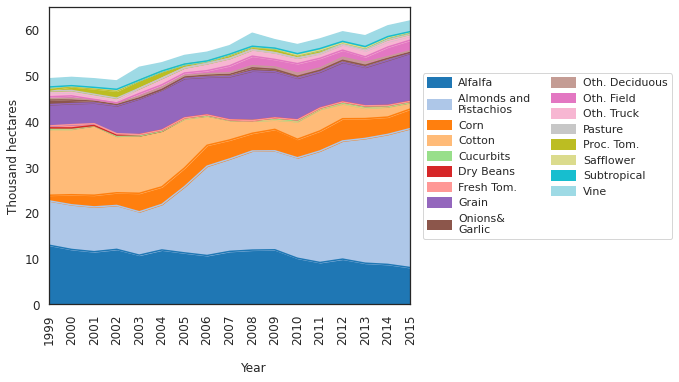
\includegraphics[width=0.6\textwidth]{land_hist_semitropic.png}
    \caption{Historical cropland of Semitropic WSD}
    \label{fig:m1esh1}
\end{figure}

\subsection{Yield Elasticity to Water}

Crop yield elasticity to water ($\tilde{y}_{i,water}$) represents the response of yield to changes in water applied, as percent change in yield to a percent change in applied water. To estimate this parameter we used two approaches, first for crops Alfalfa, Corn, Almonds (in Almonds and Pistachios category), and Wheat (in Grain category) we used the VIC-CropSyst model (\cite{malek_viccropsyst-v2_2017}) calibrated for a spatial grid in the study area and using different irrigation systems. Crop yield responses were estimated by reducing applied water (deficit irrigation), responses from VIC-CropSyst (V-CS) were later used to estimate the crop yield water elasticity ($\tilde{y}_{i,water}$) using following a sigmoidal yield response function (Equation A.3) described by \textcite{merel_regional_2014}. We fitted the sigmoidal response function using a nonlinear regression solving for $\alpha_{i,1},\alpha_{i,2},\alpha_{i,3}$, results are shown in SI. With the estimates from solving this regression the crop-specific yield response to water changes was later calculated using Equation A.4. using the reference water applied ($\tilde{x}_{i,water}$) and reference yield ($\tilde{y}_{i}$) used in the PMP calibration (average of the historical). 

\begin{flalign}
\hat{y}_{i,V-CS} = \dfrac{\alpha_{i,1}}{1 + exp\left(-\dfrac{\hat{x}_{i,water,V-CS}-\alpha_{i,2}}{\alpha_{i,3}}\right)}
\end{flalign}

\begin{flalign}
\tilde{y}_{i,water} = \dfrac{\tilde{x}_{i,water}exp\left(-\dfrac{\tilde{x}_{i,water}-\bar{\alpha}_{i,2}}{\bar{\alpha}_{i,3}}\right)\hat{y}_{i}}{\bar{\alpha}_{i,1}\bar{\alpha}_{i,3}}
\end{flalign}

For the rest of the crops we used the applied water by crop category from \textcite{dwr_agricultural_2020} and yield from the most representative crop within each group using the land reported by \textcite{usda_national_2020}, both reported at a county level and using the data from 1998 to 2015. We estimated the elasticity through least squares (Equation A.5) as the slope between the natural logarithm of production and the natural logarithm of water used. We compared our results with other published values for crops in California, specially for San Joaquin Valley (\cite{garnache_social_2017,merel_regional_2014}). Results of both approaches are summarized in SI.   

\begin{flalign}
ln(\tilde{y}_{i,t}) = \tilde{y}_{i,water}ln(\tilde{x}_{i,water,t})
\end{flalign}



\subsection{Groundwater Pumping Cost}

The unitary (\$1/$m^3$) pumping cost $\omega_{GW}$ is given by the Equation 34, where $\omega_{pump}= \$200,000$ is the capital cost of the well pump, $A_{service}=80$ ha is the assumed pumping service area, $\widetilde{x}_{water}=4,933 m^3/ ha$ is the assumed average irrigation demand per unit area, $i=0.05$ is the discount rate, $n=20$ is the pump years lifetime, $\zeta= \$6.6\times10^{-5} /m^3 m$ is the variable operation and maintenance costs for the pump, $\omega_{E,t} \$/kWh$ is the price of electricity, $\eta_{pump}=0.7$ is the average pump efficiency, $GWD_t$ is the potentiometric depth (meters) of the irrigation district in the year $t$, Q is the assumed pumping rate $0.1261 m^3/s$, C is the Hazen-Williams coefficient, pipe is assumed to be cast-iron or steel for which C = 0.12680, and $d=0.4 m$ is the pipe diameter.

\begin{equation}
\begin{gathered}
\omega_{GW,t} = \left( \dfrac{\omega_{pump}}{A_{service} \widetilde{x}_{water}} \dfrac{i(1+i)^n}{(1+i)^n-1}\right) 
+ \left(\zeta+\dfrac{\omega_{E,t}}{\eta_{pump}} \right) \left(GWD_t +10.67  \dfrac{GWD_t Q^{1.852}}{C^{1.852} d^{4.8704}}\right)
\end{gathered}
\end{equation}            

\setcounter{figure}{0} 
\setcounter{equation}{0} 
\setcounter{table}{0} 


\section{Calibration Groundwater Depth Response Function}

As explained in Section 3.2 we used the difference between the groundwater depth at the beginning of the water year and groundwater depth at the end of the water year ($\Delta{GWD}$) and groundwater pumping to calibrate a response function. Figure B.1 shows the evolution of changes of depth to the groundwater from simulation results of C2VSIM-FG from 1974-2014 simulation years that were used for the calibration of the response function. 



\begin{figure}[H]
\centering
    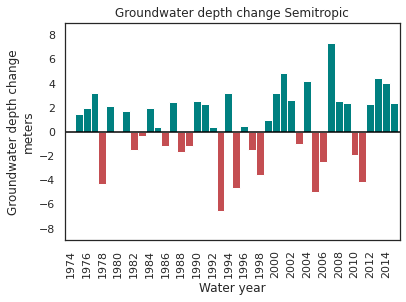
\includegraphics[width=0.4\textwidth]{Depth_change_semitropic}
    \label{fig:mesh1}
    \caption{Changes on distance to groundwater depth from C2VSIM-FG}
\end{figure}


Using groundwater pumping of the year $t$ and $t-1$ and water year type (Wet, Normal and Dry) of the year $t$ and $t-1$ as index variables we fitted different Bayesian linear modes. Pooled model (or fixed-effects) assigns same model parameters (intercept and slopes) across water year types. Un-pooled model assigns different parameters to each water year type as if water-year type is independent and have different intercepts and slopes. Finally, the Hierarchical model (or random-effects or multi-level) assigns different parameters to each water-year type varying intercepts or slopes (or both) across water-year type categories, this models enables the statistical model to learn how the agricultural pumping affects the groundwater depth change in each water year type while learning this effect from all the water wear types at the same time. Groundwater pumping ($GWP_{t}$, $GWP_{t-1}$) and change of depth to groundwater ($\Delta{GWD}_t$) were normalized using the z-score normalization. Bayesian modeling uses a maximum entropy distribution to define the likelihood of the output, for this study we use Student's-t distribution to model the groundwater depth change probability distribution. The characteristics of the Student's t distribution makes it a more robust distribution to include extreme values and that can improve the MCMC sampling process. Additionally we need to define priors of the parameters (or unobserved variables). For this study we defined Gaussian priors for the intercept and slopes in all the model variations. As we expect that the relationship between groundwater depth change and change being positive for which case we centered the Gaussian distribution on the positive side for ${GWP}_t$ and a less informative distribution centered in 0 for ${GWP}_{t-1}$. Additionally an exponential distribution for the standard deviation priors  and Gamma distribution for the degrees of freedom of the Student-t's distribution prior.  The different models variations with their respective linear model are: 

\begin{itemize}[noitemsep,topsep=0pt,parsep=0pt,partopsep=0pt]
  \item P1: Pooled,   $\mu_t = \alpha + \beta_{1}GWP_{t}$
  \item P2: Pooled with lag on pumping,   $\mu_t = \alpha + \beta_{1}GWP_{t} + \beta_{2}GWP_{t-1} $
  \item U1: Unpooled, $\mu_t = \alpha_{WY_{t}} + \beta_{1,WY_{t}}GWP_{t}$
  \item U2: Unpooled with lag on pumping, $\mu_t = \alpha_{WY_{t}} + \beta_{1,WY_{t}}GWP_{t} + \beta_{2,WY_{t}}GWP_{t} $
  \item U3: Unpooled with lag on pumping and slope, $\mu_t =  \alpha_{WY_{t}} + \gamma_{WY_{t-1}} + \beta_{1,WY_{t}}GWP_{t} + \beta_{2,WY_{t}}GWP_{t}$
  \item H1: Hirerarchical with varying intercept, $\mu_t = \alpha_{WY_{t}} + \beta_{1}GWP_{t}$
  \item H2: Hirerarchical with varying intercept and varying slope, $\mu_t = \alpha_{WY_{t}} + \beta_{1,WY_{t}}GWP_{t}$
  \item H3: Hirerarchical with varying slopes, $\mu_t = \alpha_t + \beta_{1,WY_{t}}GWP_{t} + \beta_{2,WY_{t}}GWP_{t}$
  \item H4: Hirerarchical with varying intercept and slopes, $\mu_t = \alpha_{WY_{t}} + \beta_{1,WY_{t}}GWP_{t} + \beta_{2,WY_{t}}GWP_{t}$
  \item H5: Hirerarchical with varying intercepts and slopes, $\mu_t = \alpha_{WY_{t}} + \gamma_{WY_{t-1}} + \beta_{1,WY_{t}}GWP_{t} + \beta_{2,WY_{t}}GWP_{t}$
\end{itemize}


Model variations were sampled using the No-U-Turn Sampler (NUTS) (\cite{homan_no-u-turn_2014}), a variation of the Hamiltonian Monte Carlo algorithm, and using four chains implemented with the Python package PyMC3  (\cite{salvatier_probabilistic_2016}). We coded the model variations following a non-centered parameterization to avoid divergent transitions in the sampling process (\cite{mcelreath_statistical_2020}). The LOO-CV validation results are summarized in the Figure B.2. Where the best model for Semitropic is a the hirerarchical model with varying intercepts and slopes and the pooled with lag on pumping model for Westlands. Equations B.1 describe the H5 model selected for Semitropic which results are summarized in Table B.1. Finally Equations B.2 describe the P2 model selected for the groundwater depth response function for Westlands, results are summarized in Table B.2.

\begin{figure}[H]
\centering
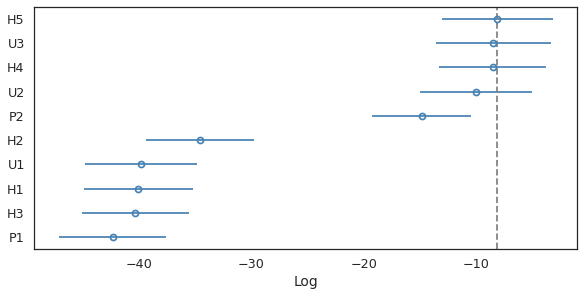
\includegraphics[width=0.7\textwidth]{model_comparison_calibration.png}
\label{fig:mesh1}
\caption{Leave-one-out cross-validation results}
\end{figure}


\begin{flalign}
\Delta & GWD_{t} \sim Student \mh t(\mu_{t},\sigma,\nu) & \notag\\
\mu_t & = \alpha_{WY_{t}} +  \gamma_{WY_{t-1}} + \beta_{1  WY_{t}}GWP_{t} + \beta_{2  WYR_{t-1}} GWP_{t-1} \notag\\
\alpha_j & = Normal(0 ,0.5)\notag\\
\gamma_j & = Normal(0,0.5)\notag\\
\beta_{1j} & = Normal(0.5,0.5) \hspace{1em}  for j = \{Wet,Normal,Dry\} \notag\\
\beta_{2j} & = Normal(0,0.5) \notag\\
\sigma & = Exponential(1) \notag\\
\nu & = Gamma(2,0.1)\notag
\end{flalign}


\begin{center}
\begin{tabular}{ |c|c|c|c|c| }
 \hline
 Parameter & Mean & Sd & HDI $2.5\%$ & HDI $97.5\%$ \\ 
 \hline
$\alpha_{1[Wet_{t}]}$ & 	-0.063 &	0.232 &	-0.478 &	0.405 		 \\
$\alpha_{1[Normal_{t}]}$ & 0.041 &	0.223 &	-0.379 &	0.501 	 \\
$\alpha_{1[Dry_{t}]}$ & 	 0.079 &	0.217 &	-0.356 &	0.494	 \\
$\gamma_{1[Wet_{t}]}$ & 	-0.057 	& 0.224 &	-0.481 &	0.393 	 \\
$\gamma_{1[Normal_{t}]}$ & 0.159 &	0.225 &	-0.285 &	0.588 \\
$\gamma_{1[Dry_{t}]}$ & 	 	-0.041 &	0.217 &	-0.453 &	0.400 	 \\
$\beta_{1[Wet_{t \mh 1}]}$ & 	 	1.207 &	0.107 &	0.995 &	1.419 	 \\
$\beta_{1[Normal_{t \mh 1}]}$ 	& 0.829 &	0.148 &	0.550 &	1.126	\\
$\beta_{1[Dry_{t \mh 1}]}$ & 0.817 &	0.088 &	0.649 &	0.991 \\
$\beta_{2[Wet_{t \mh 1}]}$ & 	-0.757 	& 0.100 & -0.940 & 	-0.551 	 \\
$\beta_{2[Normal_{t \mh 1}]}$ 	& -0.807 &	0.141 &	-1.094 &	-0.543 	\\
$\beta_{2[Dry_{t \mh 1}]}$ & 	-0.336 	& 0.088 & 	- 0.507 &  -0.159 \\
$\sigma$ & 0.235 & 	0.037 & 	0.169 & 	0.310 \\
$\nu$ 	& 20.470 & 	12.859 & 2.469 &  	45.244 \\
\hline
\end{tabular}
\captionof{table}{Marginal posterior distributions of the parameters of Groundwater Depth Response for Semitropic}
\end{center}


\newpage
\printbibliography

\end{document}

\textbf{abstract AGU}


Model    
% $$\Delta GWD \sim Normal(\mu_{i},\sigma)$$

% $$\mu_i = \alpha_{water \, year_{t}[i]} + \gamma_{water\, year_{t-1}[i]} + \beta_{water\, year_{t}[i]}*AGWP_{[i]} + \beta2_{water\, year_{t-1}[i]}*AGWP_{[i]}$$

% $$\alpha_{[i]} \sim Normal(\overline{\alpha},\sigma_{\alpha})$$

% $$\gamma_{[i]} \sim Normal(0,\sigma_{\gamma})$$

% $$\beta_{[i]} \sim Normal(\mu_{\beta},\sigma_{\beta})$$

% $$\beta_{[i]} \sim Normal(0,\sigma_{\beta})$$


% $$\alpha[i] \sim Normal(0,1)$$

% $$\alpha[i] \sim Normal(0,1)$$

% $$\alpha[i] \sim Normal(0,1)$$

% $$\alpha[i] \sim Normal(0,1)$$

\begin{center}
\begin{tabular}{ |c|c|c| } 
 \hline
 Parameter & Description & Source \\ 
 $b_{SW,t}$ & Surface water available for each year t & \cite{zeff_californias_2020} \\ 
 $p_{i,t}$ & Prices by crop i and year t & cell3 \\ 
 cell4 & cell5 & cell6 \\ 
 cell7 & cell8 & cell9 \\ 
 \hline
\end{tabular}
\captionof{table}{Parameters sampled for the stochastic time series and used in the Hydro-economic model}
\end{center}